\documentclass[a4paper,10pt]{article}
\usepackage{graphicx}
\usepackage[english]{babel}
\usepackage{geometry}           
\geometry{letterpaper}                   
\usepackage{graphicx}
\usepackage{amsmath}
\usepackage{amssymb}
\usepackage{wrapfig}
\usepackage[section]{placeins}
\usepackage{fontspec,xltxtra,xunicode}
\title{Three-Dimensional Vizualization and Animation\\Technical Report - Assignment I.}
\author{
  Marfeychuk, Mykhaylo\\
  \texttt{ist194039}
  \and
  Skalický, Matyáš\\
  \texttt{ist194904}
  \and
  Eichler, Bernardo\\
  \texttt{ist177988}
}

\date{} % 31.10.2019

\begin{document}
\maketitle

\section{Overall project structure}
The main class which is responsible for managing all of the game is the GameManager. The GameManager is created and initialized from the \textit{main.cpp} and all of the game logic is done there. But first we initialize GLUT, GLEW, and create a window. Functions of the GameManager such as keyboard inputs, mouse handling, screen resizing and rendering are registered as GLUT callbacks.

All game elements inherit from the base GameObject class. This class stores the position of the object and defines several virtual functions. For example, objects which are dynamic (DynamicGameObject) then override some of the virtual functions (such as render or update) in order to add further functionality. Other example is the CollidableGameObject which implements collisions. Full GameObject inheritance tree is visualized on the Figure below.

\begin{figure}[!htb]
	\centering
  	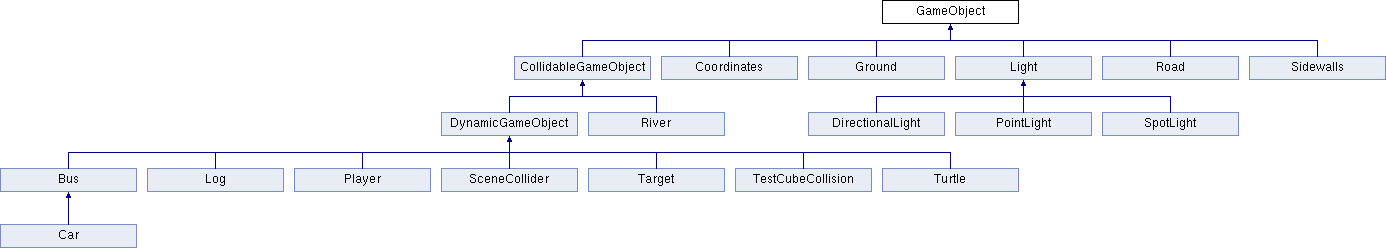
\includegraphics[width=\linewidth]{images/image1.png}
  	\caption{Objects which inherit from the GameObject class.}
\end{figure}

GameManager class is responsible both for storing and updating all of the GameObjects. All of the objects in the scene are stored in a vector inside the GameManager. When the class is initialized, an init function is called for each of them. Init function is responsible for setting up of materials and allocation of all of the meshes for each object. Since all of the meshes are stored in a global array, instead of manually typing the meshID's, we utilize a static ID counter attached to the GameObject class which dynamically keeps track of mesh IDs.

Each render pass (automatic callback from GLUT) first all of the physics are updated. All of the GameObjects implement an update function. In case of DynamicGameObject, this function is overriden to actually change the position of the GameObject. All of the updates are multiplied by a deltaTime variable in order to preserve the game speed even with varying FPS. After the physics update, we check for collisions between the player and the environment as well as between some of the moving objects in the scene and side colliders. If the GameObject is out of the scene, we move it to the other side of the map.

Last step of each render pass is to call render function on all of the GameObjects. This function is responsible for transforming, rotating and scaling of all of the meshes in the game and then sending them into the graphics pipeline. 

As the player progresses, the score as well as game difficulty increases. This is done by multiplying all of the environment's movements by a global multiplier variable.

\section{Graphic modeling}
All of the game objects are created out of cube meshes with different materials. Busses and cars have animated wheel movements, the turtles dynamically move above and under the water and logs are moving in the water flow.

\section{Cameras}
All of the Cameras inherit from the GameObject class. This allows us to easily change their position. User can switch different cameras with keyboard shortcuts. The position of the camera which follows the player is updated from the GameManager class after each physics pass.

\begin{figure}[!htb]
	\centering
  	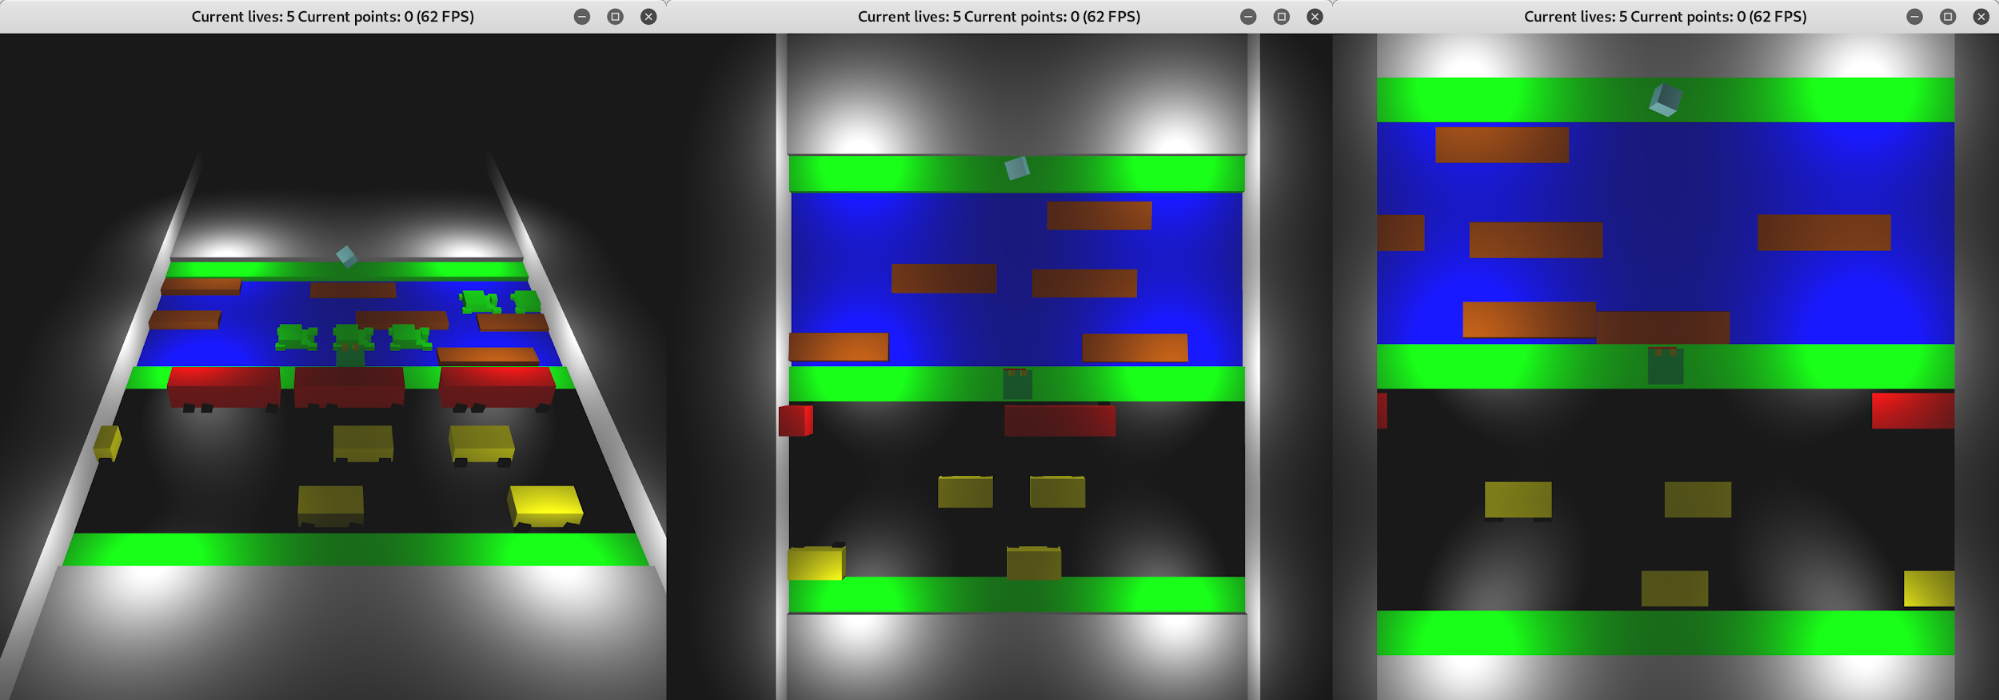
\includegraphics[width=\linewidth]{images/image6.png}
  	\caption{From left to right: perspective moving, perspective fixed and orthogonal camera.}
\end{figure}

\section{Movement of game elements}
All of the moving GameObjects inherit from the DynamicGameObject class. This class extends the GameObject class with speed vector. Each physics update, this vector is multiplied by deltaTime and added to the current GameObject's position. $$\text{position} = \text{position} + \text{deltaTime} \cdot \text{speed}$$

\section{Lighting of the scene}
All of the lights inherit from the GameObject class. The position of the GameObject is used as the position of the light. In case of SpotLight, we also use another vector to store the direction of the light. All of the positions of lights are passed as individual uniforms into the vertex and later fragment shader. This could be improved with usage of vertex buffer objects, however our solution works well for a project of this scale.

Based on the state of the light (ON/OFF), all of the colors of fragments are summed in the fragment shader. We used the code provided from exercises but modified if for our usecase. We have also consulted the Redbook in order to implement different types of lights.

\begin{figure}[!htb]
	\centering
  	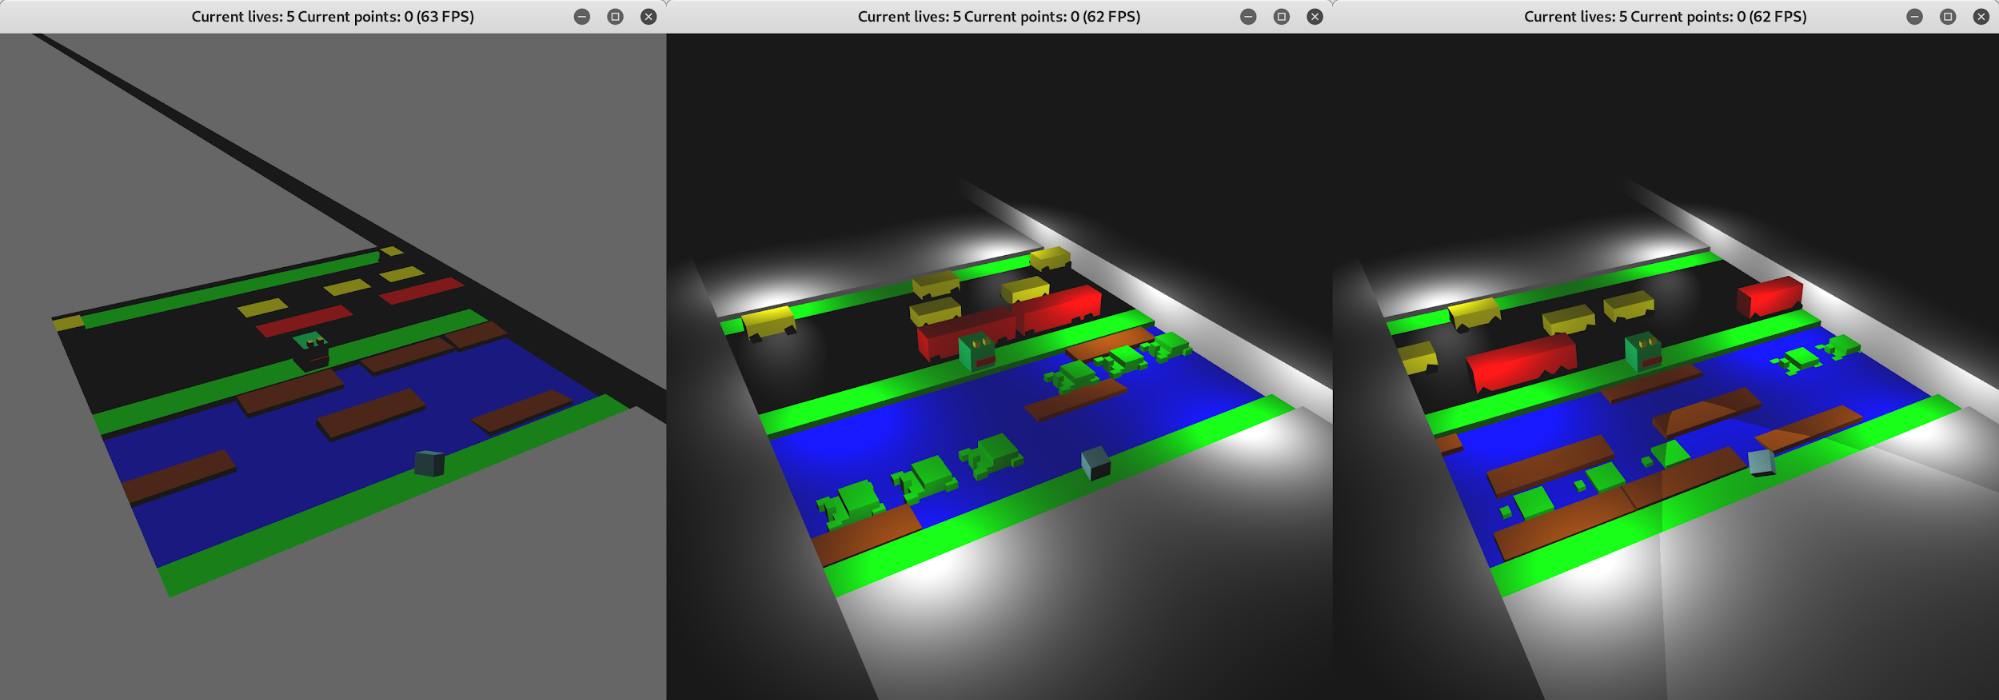
\includegraphics[width=\linewidth]{images/image3.png}
  	\caption{From left to right: directional light, point lights and point lights with spotlight.}
\end{figure}

\section{Collision detection}
After each physics update, the collisions are checked by the GameManager class. All of the collidable GameObjects contain a bounding box and also a function to check for collisions between them. Since we do not need to check collisions between all of the GameObjects within the scene, we can save resources and need to only perform O($n$) comparisons instead of O($n^{2}$).

\begin{figure}[!htb]
	\centering
  	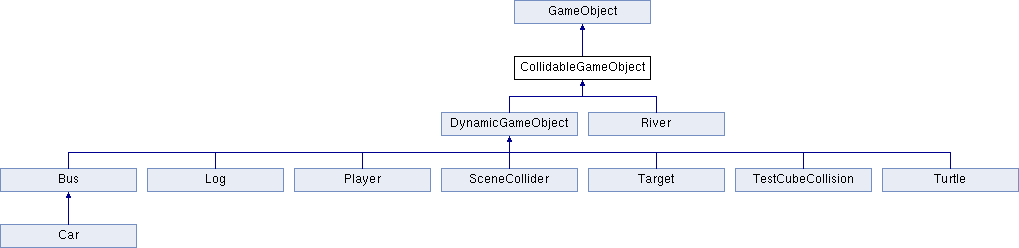
\includegraphics[width=\linewidth]{images/image5.png}
  	\caption{All of the collidable game objects in the game.}
\end{figure}

In order to check what's beneath of the player, the player's GameObject contains 2 colliders. One on the top for collisions with cars and busses and one beneath to check whether the player is standing on a log or a turtle.

\section{Texture mapping}
Due to time constraints of our team members, texture mapping was not implemented at the date when the project was showcased in the lab. However we have \emph{implemented the texturing} while this report was also written. The textures are handled using the TGA texture class.
\begin{figure}[!htb]
	\centering
  	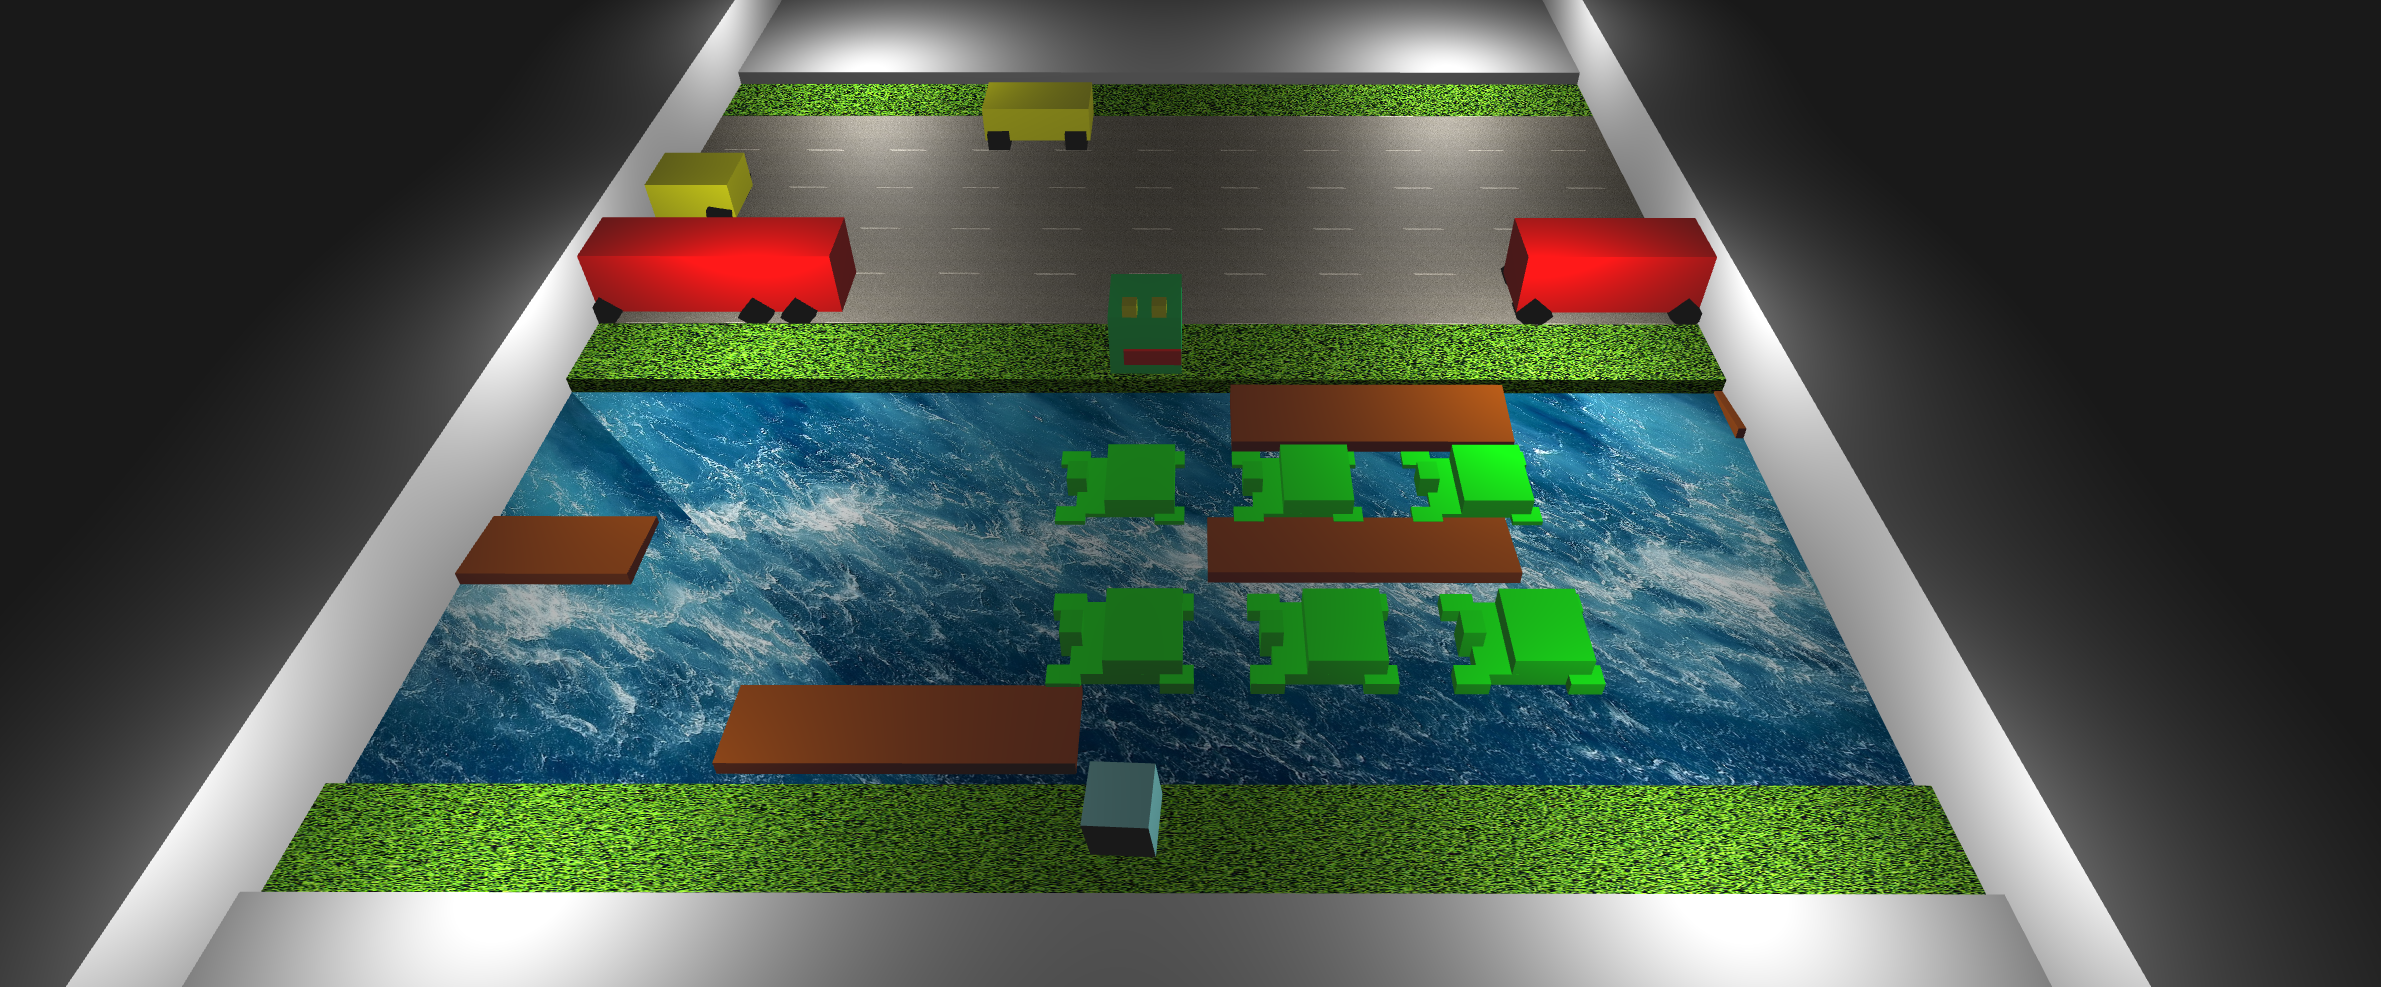
\includegraphics[width=0.85\linewidth]{images/textures.png}
  	\caption{Textures in the game.}
\end{figure}


\section{HUD (lives, score, reset, pause)}
We utilized the game window's title to communicate with the player. This is done by accessing the GLUT's window handle and passing a string into it. Game window therefore shows the information about the current lives, score and provides the user with instructions when the player dies. This can be seen on the image below.

\begin{figure}[!htb]
	\centering
  	
\includegraphics[width=\linewidth]{images/image2.png}
\end{figure}


\section{Conclusion}
We have implemented a functional prototype of a Frogger3D game in OpenGL. Matyáš Skalický is responsible for the overall architecture, physics and lights. Mykhaylo Marfeychuk worked on collision detections, object modeling, respawning, animation and texturing. Bernardo Eichler was not able to contribute to this assignment due to personal reasons. We hope that this will be not the case of the following assignments. Since the showcase of the project at the laboratory, we have implemented the missing textures.

\end{document}  